\documentclass{article}
\usepackage{amsmath, amssymb, amsthm}
\usepackage{mathtools}      % For \coloneqq and other extensions
\usepackage{algorithm}
\usepackage{algpseudocode}
\usepackage{booktabs}       % For nice tables
\usepackage{array}
\usepackage{graphicx}
\usepackage{xcolor}
\usepackage{hyperref}
\usepackage{enumitem}       % For customized lists
\usepackage{tikz}
\usetikzlibrary{arrows.meta, positioning}

% ============================================================================
% THEOREM ENVIRONMENTS
% ============================================================================
\theoremstyle{plain}
\newtheorem{theorem}{Theorem}[section]
\newtheorem{lemma}[theorem]{Lemma}
\newtheorem{proposition}[theorem]{Proposition}
\newtheorem{corollary}[theorem]{Corollary}

\theoremstyle{definition}
\newtheorem{definition}[theorem]{Definition}
\newtheorem{example}[theorem]{Example}
\newtheorem{remark}[theorem]{Remark}

% ============================================================================
% CUSTOM COMMANDS FOR NOTATION
% ============================================================================
% Bit operations (matching Hamilton's notation)
\newcommand{\XOR}{\oplus}           % XOR: exclusive or
\newcommand{\AND}{\mathbin{\wedge}}            % AND
\newcommand{\OR}{\mathbin{\vee}}               % OR
\newcommand{\NOT}{\mathord{\sim}}              % NOT (bitwise complement)
\newcommand{\SHL}{\mathbin{\triangleleft}}     % Shift left
\newcommand{\SHR}{\mathbin{\triangleright}}    % Shift right
\newcommand{\ROTL}{\mathbin{\circlearrowleft}} % Rotate left
\newcommand{\ROTR}{\mathbin{\circlearrowright}}% Rotate right
\newcommand{\vplus}{\mathbin{\oplus}}   % plus
\newcommand{\vtimes}{\mathbin{\otimes}}

% Convenient shortcuts
\newcommand{\gc}{g}                  % Gray code function
\newcommand{\gcinv}{g^{-1}}          % Gray code inverse
\newcommand{\bitfn}{\mathrm{bit}}              % bit extraction function
\newcommand{\tsb}{\mathrm{tsb}}                % trailing set bits
\newcommand{\entry}{e}                % entry point function
\newcommand{\exitpt}{f}               % exit point function (f for "finish")
\newcommand{\dir}{d}                  % direction function
\newcommand{\gcr}{\mathrm{gcr}}                % Gray code rank
\newcommand{\order}{m_{\text{max}}}
\newcommand{\dk}{dk}
\newcommand{\embed}{\kappa}
% Sets
\newcommand{\Z}{\mathbb{Z}}                    % Integers
\newcommand{\N}{\mathbb{N}}                    % Natural numbers
\newcommand{\B}{\mathbb{B}}                    % Binary digits {0,1}

% Other
\newcommand{\encode}{\mathrm{encode}}
\newcommand{\decode}{\mathrm{decode}}


\title{Lattice-Continuous Compact Hilbert Indices via Affine Transformations on Hypercubes}
\author{Andrew Dolgert}
\date{\today}


\begin{document}
\maketitle
\begin{abstract}
Space-filling curves are fundamental to combinatorial optimization and multidimensional indexing.
Existing compact linearizations for unequal dimensions fail to preserve lattice continuity (adjacency), degrading locality.
We introduce a general construction using Gray codes and affine transformations in $\mathbb{F}_2^n$.
We prove this construction yields a lattice-continuous mapping for arbitrary dimension extents and provide an $O(mn)$ time algorithm.
\end{abstract}
\section{Introduction}

Space-filling curves are fundamental to combinatorial optimization and multidimensional indexing. For Compact Hilbert indices:
\begin{itemize}
    \item Vision transformers (ViT) and image flattening for AI.
    \item 3D point cloud analysis for 3D LiDAR data.
    \item Efficient nearest-neighbor search. This is used in vector databases like Pinecone or Milvus that power modern RAG. Eg., Approximate nearest neighbor or Hilbert R-trees.
    \item Malware classification (visual analysis) - Researchers convert binary executables into images to train CNNs for malware detection.
    \item Adaptive mesh refinement in CFD/Physics. Libraries like libMesh use CHC concepts to reorder mesh elements in memory in order to improve cache locality.
    \item Genome Sequence Analysis - DNA sequences have arbitrary lengths. For comparison, CHC allows projecting multi-dimensional k-mer frequencies into 1D arrays.
\end{itemize}


\begin{center}
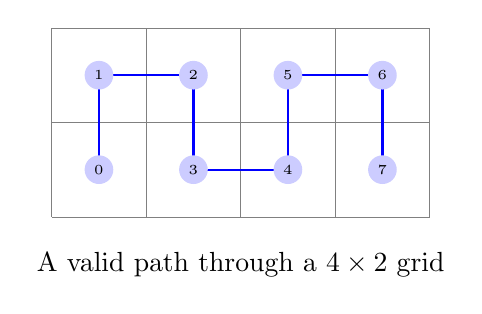
\begin{tikzpicture}[scale=1.2]
    \draw[step=1, gray, very thin] (0,0) grid (4,2);
    % A valid Hilbert-like path
    \draw[thick, blue, ->]
        (0.5,0.5) -- (0.5,1.5) -- (1.5,1.5) -- (1.5,0.5) --
        (2.5,0.5) -- (2.5,1.5) -- (3.5,1.5) -- (3.5,0.5);
    \foreach \x/\y/\n in {0.5/0.5/0, 0.5/1.5/1, 1.5/1.5/2, 1.5/0.5/3,
                          2.5/0.5/4, 2.5/1.5/5, 3.5/1.5/6, 3.5/0.5/7} {
        \node at (\x,\y) [circle, fill=blue!20, inner sep=2pt] {\tiny \n};
    }
    \node at (2, -0.5) {A valid path through a $4 \times 2$ grid};
\end{tikzpicture}
\end{center}
\begin{center}
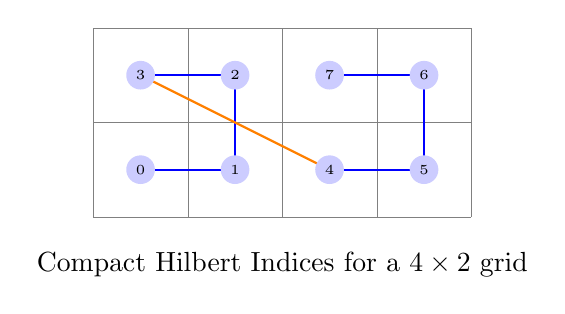
\begin{tikzpicture}[scale=1.2]
    \draw[step=1, gray, very thin] (0,0) grid (4,2);
    % A valid Hilbert-like path
    \draw[thick, blue, ->]
        (0.5,0.5) -- (1.5,0.5) -- (1.5,1.5) -- (0.5,1.5);
    \draw[thick, blue, ->]
        (2.5,0.5) -- (3.5,0.5) -- (3.5,1.5) -- (2.5,1.5);
    \draw[thick, orange, ->]
        (0.5,1.5) -- (2.5,0.5);
    \foreach \x/\y/\n in {0.5/0.5/0, 1.5/0.5/1, 1.5/1.5/2, 0.5/1.5/3,
                          2.5/0.5/4, 3.5/0.5/5, 3.5/1.5/6, 2.5/1.5/7} {
        \node at (\x,\y) [circle, fill=blue!20, inner sep=2pt] {\tiny \n};
    }
    \node at (2, -0.5) {Compact Hilbert Indices for a $4 \times 2$ grid};
\end{tikzpicture}
\end{center}

Existing compact linearizations for unequal dimensions fail to preserve lattice continuity (adjacency), degrading locality.
$$
    ||x-y||_1 = 1 \implies ||H(x)-H(y)||_1=1
$$
\begin{definition}[Lattice Continuity]
A space-filling curve $H: \mathcal{D} \to \mathbb{Z}$ is lattice-continuous if for any two points $p, q \in \mathcal{D}$ with Euclidean distance $||p-q||_1 = 1$, the difference in their index $|H(p) - H(q)|$ is minimal.
\end{definition}

This continuity can be helpful for
\begin{itemize}
    \item Using Hilbert curves to define bounding boxes.
    \item Using Hilbert curves for locality... I'll need to measure this.
    \item Using space-filling curves for CNC milling and laser cutting or for 3D printing.
    \item Data compression with change codes that encode only the next step direction.
    \item Image processing with the Riemersma dithering technique. You get jumps.
    \item Topological algorithms that detect connected components, as in ``find all connected cloud pixels''. Standard Hilbert also fragments regions, but lack of lattice continuity complicates stitching.
\end{itemize}
(There are Scan-line and Gilgamesh variants that are used for arbitrary rectangles for CNC.)

We introduce a general construction using Gray codes and affine transformations in $\mathbb{F}_2^n$.
We prove this construction yields a lattice-continuous mapping for arbitrary dimension extents and provide an $O(mn)$ time/space algorithm.


\section{Preliminaries}
Hilbert curves are traditionally built using nested sequences of $n$-dimensional
cubes. The space of the binary Galois Field $V_k=\mathbf{F}_2^k$ is a natural fit.
It is equipped with an XOR for addition, which we label $\vplus$ and
an AND for multiplication, which we label $\vtimes$.

Critical to the Hilbert construction are Gray codes which are Hamiltonian
paths on the corners of the $k$-dimensional cube $Q_k\{0,1\}^k\cong\mathbf{F}_2^k$.
We can consider a Gray code a transform from $G:\mathbf{F}_2^k\rightarrow \mathbf{F}_2^k$
if we convert integers $\mathcal{I}_n=\mathbb{Z}_{2^k}$ using natural binary
code $B:\mathcal{I}_n\rightarrow V_k$.
We restrict ourselves to Gray codes that start at the origin of $V_k$ and
map the last index $2^{n-1}$ to the axis $\epsilon_0$\cite{alber2000multidimensional}.

A binary Gray code guarantees that only one index changes at a time.
$$
    G(B(i))\XOR G(B(i+1)) = \epsilon_{g(i)}
$$

Consider a point in $n$-dimensions where each dimension has extent $2^m$.
A Hilbert curve defines a bijection $\mathcal{H}: (\mathbb{Z}_{2^m})^n\rightarrow \mathbb{Z}_{2^{nm}}$. The order of the curve is $m$.
We consider Hilbert curves that map $0$ to $\mathbf{0}$ and $2^{mn}$ to $(2^m-1)\epsilon_0$ along the 0-axis.

\section{Construction of Hilbert Curves}

\subsection{Introduction}
While there are many Hilbert curves\cite{haverkort2016many}, we will consider
only constructions that follow a nested compositional framework across $m$ levels. This framework addresses each level as a partitioning of the space
into a dyadic cube $Q_k$ and for each partitioning requires two definitions.
\begin{enumerate}
    \item A Gray code as described above.
    \item A set of affine transforms to apply to every element of $Q_k$ at the next level.
\end{enumerate}
The Gray code assures adjacency at this level. The affine transforms rotate
child Gray codes so that, were they to assure adjacency within the child,
they would remain adjacent.
Gray codes can be generated by construction\cite{haverkort2016many}, by induction\cite{hamilton2008compact}, by permutation languages (cite), or by search. (The file hypercubes\_lec10.pdf has references I may need to cite.)

The set of affine transforms has often been found by symmetry considerations.
We offer an algorithm here to enumerate the allowed affine transforms that
result in a lattice-continuous Hilbert curve.

While a general permutation of a child is possible, we are concerned with
ensuring that the child's Gray code, which we have required to have
an origin at $0$ and an exit at $\epsilon_0$, is oriented in a particular
direction. The possible orientations on $Q_k$ are enumerated by all
rotations and translations, as shown below, which allows us to focus on
affine transformations using a cyclic rotation $\rho^d$ of axes by $d$ and translation by $e$.
$$
    S_{e,d}(y) = \rho^d y + e
$$

\subsection{Affine transforms and rotations}
\begin{theorem}
Let $n \ge 1$. The set of affine transforms $\{S_{e,d} : e \in \mathbb{F}_2^n,\, d \in \mathbb{Z}_n\}$
is in bijection with the set of directed edges of the $n$-dimensional hypercube.
\end{theorem}

\begin{proof}
Let $V = \mathbb{F}_2^n$ be the vector space over $\mathbb{F}_2$ with standard basis
$\{\mathbf{e}_0, \ldots, \mathbf{e}_{n-1}\}$.
The vertices of the $n$-cube are the elements of $V$, and two vertices are adjacent
if and only if they differ by some $\mathbf{e}_a$.

A \emph{directed edge} is an ordered pair $(u, u + \mathbf{e}_a)$ where $u \in V$ and $a \in \mathbb{Z}_n$.

\medskip
\noindent\textbf{Counting.}
There are $2^n$ choices for $u$ and $n$ choices for $a$, giving $n \cdot 2^n$ directed edges.
There are $2^n$ choices for $e$ and $n$ choices for $d$, giving $n \cdot 2^n$ transforms.

\medskip
\noindent\textbf{The transform.}
Let $\rho \in \mathrm{Sym}(\mathbb{Z}_n)$ be the cyclic permutation $\rho(a) = (a+1) \bmod n$,
acting on $V$ by $(\rho \cdot v)(a) = v(\rho^{-1}(a))$.
Then $\rho \cdot \mathbf{e}_j = \mathbf{e}_{(j+1) \bmod n}$.

Define $S_{e,d} : V \to V$ by
$$
S_{e,d}(x) = \rho^{d} \cdot x + e.
$$
The inverse is $S_{e,d}^{-1}(y) = \rho^{-d} \cdot (y + e)$.

\medskip
\noindent\textbf{Reference edge.}
Fix the directed edge $R = (\mathbf{0}, \mathbf{e}_{0})$ as the reference.
Under $S_{e,d}$:
\begin{align*}
S_{e,d}(\mathbf{0}) &= e, \\
S_{e,d}(\mathbf{e}_{0}) &= \mathbf{e}_{d} + e.
\end{align*}
Thus $S_{e,d}$ maps $R$ to the directed edge from $e$ along axis $d$.

\medskip
\noindent\textbf{Surjectivity.}
Given any directed edge $(u, u + \mathbf{e}_a)$, choose
$$
e = u, \qquad d = a.
$$
Then $S_{e,d}(R) = (u, u + \mathbf{e}_a)$.

For the reverse orientation $(u + \mathbf{e}_a, u)$, choose
$$
e = u + \mathbf{e}_a, \qquad d = a.
$$
Then:
\begin{align*}
S_{e,d}(\mathbf{0}) &= u + \mathbf{e}_a, \\
S_{e,d}(\mathbf{e}_{0}) &= (u + \mathbf{e}_a) + \mathbf{e}_a = u.
\end{align*}

\medskip
\noindent\textbf{Injectivity.}
The map $S_{e,d} \mapsto S_{e,d}(R)$ sends distinct pairs $(e, d)$ to distinct
directed edges, since $e$ determines the starting vertex and $d$ determines the axis.

\medskip
\noindent\textbf{Conclusion.}
The map $S_{e,d} \mapsto S_{e,d}(R)$ is a bijection between
$\{S_{e,d}\}$ and directed edges of the $n$-cube.
\end{proof}

\begin{lemma}[Interpretation for Hilbert curves]
The state $(e, d)$ of a Hilbert curve encodes exactly the information needed to specify
an entry vertex and an exit direction. The bijection above shows this encoding is tight:
no redundancy, no missing configurations.
\end{lemma}

\subsection{Finding Correct Transforms}

\begin{enumerate}
\item For each vertex in the space of cubes of cubes
    \begin{enumerate}
        \item If that vertex neighbors the child of the next parent.
        \item Add a directed edge to this vertex from all neighbors that
        are one unit vector away and are NOT neighbors of children of the next parent.
    \end{enumerate}
    \item Add an edge from the origin to every neighbor one unit vector away.
    \item Find all paths from the origin to the exit at $(3,0,\ldots,0)$.
    \item Choose a path and for every vertex in that path, create a new graph.
    \begin{enumerate}
        \item Search all edges from the exit of one child
        \item Search the neighbors of those edges to find the exit to the next child.
        \item Add paths for every combination that connects those two. 
    \end{enumerate}
    \item Find all paths in this graph. Each one defines a set of entry and directions.
\end{enumerate}
How many paths are there? A lot. I don't know how many.

\subsection{Algorithm to Find Points and Indices}

Algorithm for point-to-index (not a surprise).

Algorithm for index-to-point (not a surprise).

Algorithm for next-index, which can generate a sequence of points in $O(1)$ time by recalculating transforms only as needed. (Maybe this is nice.
Has anybody done this before?)

\section{Affine Embedding Framework}

We start with a Hilbert curve for which we know that
$$
S^k_w(\alpha_w + \epsilon_0) + S^k_{w+1}\alpha_{w+1} = \epsilon^k_g
$$
Here the $k$ subscript says that the curve is defined in $k$ dimensions.

Given a transform specified by $e$ and $d$, we apply it during encoding with
$$
    w = \gc^{-1}(S^{-1(k)}_{e,d}(p))
$$
The transform $S^{-1(k)}_{e,d}(p)$ is an affine transform on a point $p$ in the $V_n$
space. The forward transform is a rotation and then an additon.
$$
    S^{(k)}_{e,d}(w) = \rho^d w + e
$$
The reverse is the opposite.
$$
    S^{-1(k)}_{e,d}(p) = \rho^{-d}(p + e)
$$
In $k$ dimensions a rotation is defined on $V_n$ as a rotation of the indices,
$a$, in the opposite direction.
$$
    \rho \nu(a) = \nu(\rho^{-1} a)
$$

Define a coordinate embedding transform.
$$
  \embed_{\dk}: Q_k\rightarrow Q_{k+\dk},\quad \embed_{\dk}(x_0,\ldots,x_{n-1})=(0,\ldots,0,x_0,\ldots,x_k-1)
$$
This identifies $Q_k$ with the face
$$
    F := \{y\in Q_{k+\dk}:y_0=\cdots=y_{\dk-1}=0\subseteq Q_{k+\dk} \}
$$
Because this embedding is linear over $\mathbb{F}_2$,
$$
    \embed_{\dk}\nu\vplus \embed_{\dk}\upsilon = \embed_{\dk}(\nu\vplus\upsilon),
$$
applying embedded transforms to the embedded adjacency gives a transformed
constitutive equation.
$$
    \hat{S}_{i}^{(k+\dk)}\embed_{\dk}\epsilon_0 \vplus
    \hat{S}_{i+1}^{(k+\dk)}\embed_{\dk}\mathbf{0} = \embed_{\dk}g_k(i)
$$

\section{Lattice Continuity of the Construction}


If I take an affine transform in $k$ dimensions put it into $k+\dk$ dimensions
by modifying $e$ and $d$ by putting $e$ as the high bits of a $k+\dk$ dimensional
vector and modify $d$ by increasing it by $\dk$. The embedded
transform $S'_{e',d'}$ acts on a $(k+\dk)$-bit vector $x$ as:
$$
S'_{e',d'}(x) = \rho^{d + \dk}x \oplus (\rho^{\dk}e)
$$
The new axes occupy positions $0, 1, \ldots, \dk-1$, while the original $k$
axes shift to positions $\dk, \dk+1, \ldots, k+\dk-1$. Since the new
axes have entry bit 0 (from the left-shift) and the rotation increases by $\dk$,
the transform acts as identity on the new low-order bits while preserving the original
transform's action on the high-order bits.


Remember that we assume $\epsilon_{d_i}+ e_{i}+e_{i+1} = g_k(i)$. When we
modify them as above,
$$
\begin{aligned}
    \alpha_i & = S'_i(\mathbf{0})=\rho^{\dk}e_i \\
    \omega_i & = S'_i(\mathbf{0} + \epsilon_0)=
        \rho^{d_i + \dk}\epsilon_0 + \rho^{\dk}e_{i}
        =\epsilon_{d_i+ \dk}+ \rho^{\dk} e_{i} \\
    \alpha_{i+1} & = \rho^{\dk}e_{i+1}
\end{aligned}
$$
In the $k+\dk$ dimensions this becomes:
$$
\begin{aligned}
    \omega_i + \alpha_{i+1} & = g_{(k)}(i) \\
    \epsilon_{d_i+ \dk}+ \rho^{\dk} e_{i}+\rho^{\dk}e_{i+1} & = \rho^{\dk}g_{(k)}(i)
\end{aligned}
$$
In other words, by embedding the transform that defines the child space,
we are guaranteed adjacency in that larger child space as long as the Gray step
from in the child space is an embedded version of the Gray step in the parent space.

This equation needs to apply for those indices that are used for this level,
and these are only the high $k$ active axes out of the $k+dk$ total axes. The $i$
at this level is assigned by the parent, so it runs over $[0,2^k-1]$, but that's
all that is needed during axis activation.

The final agreement we need is that, in the child layer, we need to be able to
define orientations for the children such that our boundary conditions are met
for the layer above. That is that there is an entry at the origin and an exit
at $\epsilon_0$.

For each child hypercube of the level with $k+\dk$ active dimensions, we can
use the next Gray code in the given class $\gc_{k+\dk}$.

\section{An Algorithm}
It's $\mathcal{O}(nm)$ where $n$ is the number
of dimensions and each dimension has extent $2^m$. If you consider
bit operations as handling the $n$, then it is $\mathcal{O}(m)$.


\section{Experimental Validation}

Here is the change to the spatial locality\cite{moon2001analysis}.

Gotsman-Lindenbaum Metric\cite{gotsman1996metric}.

Box-to-curve ratio (BCR)\cite{haverkort2010locality,bos2015hyperorthogonal}.

Here is the change to the bounding box problem\cite{kamel1994hilbert}.

\section{Conclusion}
We have a new algorithm to find Hilbert curves.

We have a new algorithm to generate a sequence of points ranked
by their Hilbert index.

We have a new algorithm to construct Hilbert curves of unequal side
lengths that are lattice-continuous.


\bibliographystyle{plain}
\bibliography{article}

\end{document}
